\section{Implementation}
\begin{frame}{Overview}
    \begin{itemize}
        \item Four compilation stages:
        \begin{enumerate}
            \item the lexical and syntactic analysis,
            \item semantic analysis,
            \item code generation, and % at generation time
            \item optimizations
        \end{enumerate}
        \item Process managed by a static compiler class.
        \begin{itemize}
            \item Parses command line parameters.
            \item Handles input and output of files.
            \item Calls the different stages.
            \item Handles logging and error messages.
        \end{itemize}
    \end{itemize}    
    \begin{figure}[htp]
        \centering     
        \lstinputlisting[style=bashstyle]{../figures/code/slides/cli_example.bash}
        \caption{A command line interface example.}
    \end{figure}
\end{frame}

% \begin{frame}{Symbols and Symbol Table}
%     \begin{minipage}{.45\textwidth}
%         \begin{itemize}
%             \item Symbol table used to save and propagate symbol information.
%             \item Handles higher-level concepts such as variable contexts. %! Not inherent since not functional impl.
%             \item Contains dictionary that maps identifiers to symbol objects.
%             \item All symbol objects derived from abstract symbol class.
%         \end{itemize}    
%     \end{minipage}
%     \begin{minipage}{.50\textwidth}
%         \centering
%         \begin{figure}[htp]
%             \centering
%             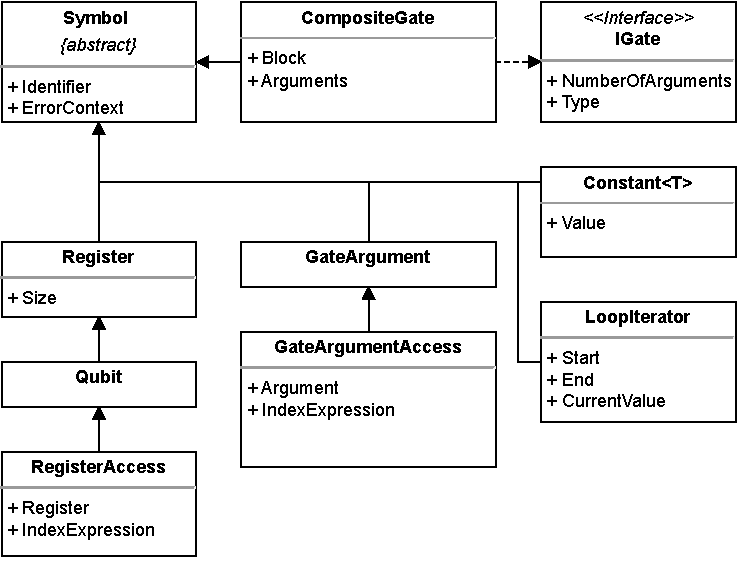
\includegraphics[]{../figures/drawio/slides/uml_symbols.pdf}
%             \caption{A diagram showing the hierarchy of symbol classes.}
%             % \label{fig:implementation_uml_errors}
%         \end{figure}
%     \end{minipage}
% \end{frame}

\subsection{Lexical and Syntactic Analysis}
\begin{frame}{Lexical and Syntactic Analysis}
    \begin{itemize}
        \item First compilation stage is lexical and syntactic analysis.
        \item Both lexer and parser created with the ANTLR4 tool.
        \item Generates the source code based on a given grammar. 
        \item Implementation of the grammar is more elaborate version of previously disused one.
    \end{itemize}
    \begin{figure}[h]
        \centering
        \lstinputlisting[style=ANTLR]{../figures/code/implementation/grammar_structure.g4}
        \caption{The basic structure of parsing rules for Luie.}
    \end{figure}
\end{frame}

\subsection{Semantic Analysis}
\begin{frame}[fragile]{Semantic Analysis}
    \begin{itemize}
        \item Analyses non-syntactic constraints of program, mainly:
        \begin{enumerate}
            \item declaration analysis and
            \item type checking.
        \end{enumerate}
        \item Declaration analysis ensures all identifiers used were previously declared and all identifiers used in declarations are not already declared.
        \item Type checking ensures that symbols are used in the correct context.
    \end{itemize}
    \vfill
    \begin{figure}[htp]
        \centering     
        \begin{lstlisting}[style=Luie, mathescape=true,basicstyle=\ttfamily\large, literate={↑}{$\aup{}$}{1}, escapechar=\%] 
qubit c;           /* $\adown$ Type error (cannot use qubits in arith. expression) */       
const regSize : int = %\uwave{c}% + 2; 
            /* $\adown$ Already declared */      
qubit[regSize] %\uwave{c}%;
              /* $\adown$ Type error (expects a register or qubit) */                      
c_h_reg c, %\uwave{a}%, %\uwave{regSize}%;
        /* ↑ Undeclared identifier */                 
        \end{lstlisting}
        \caption{Luie program with semantic errors highlighted.}
        % \label{fig:qft_example}
    \end{figure}
\end{frame}

% \begin{frame}{Semantic Analysis}
%     \begin{itemize}
%         \item This includes throwing warnings for declared but unused identifiers.
%         \item Additionally, it prevents the use of a qubit in a code block that is guarded by the same qubit because this would lead to irreversible gates.
%         \item For example, while a qubit symbol can be used as the argument for a gate application, it does not represent a classical numerical value and, therefore, cannot be used in the context of a factor.
%         \item Since we do not give the type of composite gate argument, its body cannot be type checked, and any invalid types are thrown at generation time. 
%     \end{itemize}
% \end{frame}

\subsection{Code Generation}
\begin{frame}{Code Generation}
    \begin{itemize}
        \item Parse tree is traversed and source code is translated to in-memory representation.
        \item Source code representation (SCR) is translated to target code representation (TCR).
        \item TCR can be translated directly to the textual OpenQASM code.
        \item Example code generation with program:
    \end{itemize}
    \begin{figure}
        \centering
        \lstinputlisting[style=Luie, basicstyle=\large\ttfamily]{../figures/code/implementation/codeGen_example.luie}
        \caption{An example Luie program to show the code generation process.}
    \end{figure}
\end{frame}

% \begin{frame}{Source Code Representation}
%     \begin{minipage}{.45\textwidth}
%         \begin{itemize}
%             \item All SCR objects implement the translatable interface, which requires a translation function.
%             \item The are three main translatables: the code block, statement, and declaration classes.
%             \item The block contains a list of translatables and is used for both the main block and the body of some statements.
%             \item The declaration consists only of register declarations; the compile-time-only declarations are only saved in the symbol table. 
%         \end{itemize}    
%     \end{minipage}
%     \begin{minipage}{.50\textwidth}
%         \centering
%         \begin{figure}[htp]
%             \centering
%             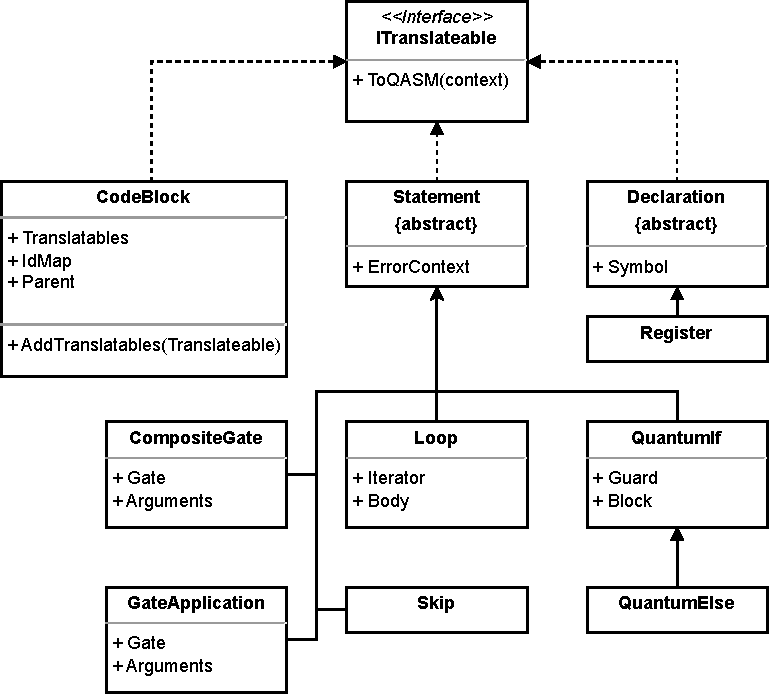
\includegraphics[]{../figures/drawio/slides/uml_translateables.pdf}
%             \caption{A diagram showing the hierarchy of translatable classes.}
%             % \label{fig:implementation_uml_errors}
%         \end{figure}
%     \end{minipage}
% \end{frame}

\begin{frame}{Source Code Representation}
    \begin{minipage}{.60\textwidth}
        \begin{itemize}
            % \item All SCR objects implement the translatable interface, which requires a translation function.
            \item Three main classes:
            \begin{enumerate}
                \item Code block: contains list of translatables.
                \item Declaration: only register declaration, constants compile-time only.
                \item Statements: variety of different classes.
            \end{enumerate}
            \item Example contains three translatables.
            \begin{itemize}
                \item First two declarations, last is gate statement.
                \item Gate's body $\supset$ if-statement $\supset$ loop statement $\supset$ gate application.
            \end{itemize}
        \end{itemize}   
        \vfill
        \begin{figure}
            \centering
            \lstinputlisting[style=Luie, basicstyle=\large\ttfamily]{../figures/code/slides/luie_example_reduced.luie}
            \caption{An example Luie program to show the code generation process.}
        \end{figure} 
    \end{minipage}
    \begin{minipage}{.35\textwidth}
        \centering
        \begin{figure}[htp]
            \centering
            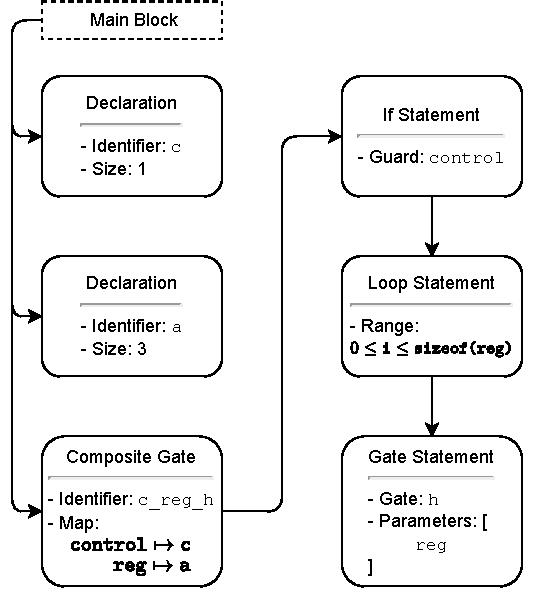
\includegraphics[]{../figures/drawio/codeGen_sourceCode_example.pdf}
            \caption{The SCR of the example program.}
            % \label{fig:implementation_uml_errors}
        \end{figure}
    \end{minipage}
\end{frame}

% \begin{frame}{Target Code Representation}
%     \begin{itemize}
%         \item The basis of the TCR is the \texttt{QASMProgram} object.
%         \item It contains a list of \texttt{Code} objects, which are either declarations of gate applications. 
%         \item All SCR objects can be translated to a list of code objects and appended to the program object.
%         \item The translations are as described in the translation section.
%         \item For example, an if-statement adds a control qubit to all gate applications in the block translation.
%         \item All code objects implement a \texttt{ToCode} function that returns the textual representation of the statement.
%         \item To translate the program object, the code objects are simply iterated, converted to text, and written to a file. 
%     \end{itemize}
%     \vfill
%     \begin{align*}        
%         ct(\texttt{qif } qArg \texttt{ do } blk \texttt{ end}, st) = \ &  control(qt(qArg, st), bt(blk, st)) \\
%     \end{align*}
% \end{frame}

\begin{frame}{Target Code Representation}    
    \begin{minipage}{.38\textwidth}
        \begin{itemize}
            \item TCR based on \texttt{QASMProgram} object.
            \item Contains list of \texttt{Code} objects, either gate or declaration. 
            \item All SCR objects translated to list of code objects and appended to program object.
            % \item The translations are as described in the translation section.
            % \item For example, an if-statement adds a control qubit to all gate applications in the block translation.
            % \item All code objects implement a \texttt{ToCode} function that returns the textual representation of the statement.
            \item Translate program object: code iterated, converted to text, written file. 
        \end{itemize}
    \end{minipage}    
    \begin{minipage}{.32\textwidth}
        \centering
        \begin{figure}[htp]
            \centering
            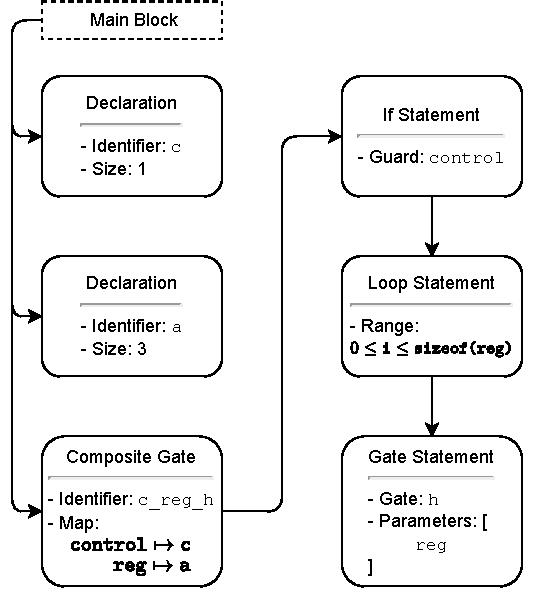
\includegraphics[width=\textwidth]{../figures/drawio/codeGen_sourceCode_example.pdf}
            \caption{The SCR of the example program.}
            % \label{fig:implementation_uml_errors}
        \end{figure}
    \end{minipage}
    \hfill
    \begin{minipage}{.28\textwidth}
        \centering
        \begin{figure}[htp]
            \centering
            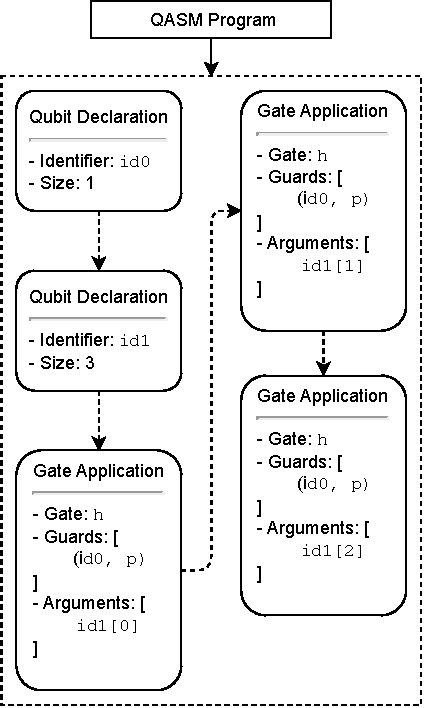
\includegraphics[width=\textwidth]{../figures/drawio/slides/codeGen_targetCode_example.pdf}
            \caption{The TCR of the example program.}
            % \label{fig:implementation_uml_errors}
        \end{figure}
    \end{minipage}
\end{frame}

\begin{frame}{Translated Example Program}    
    \begin{minipage}{.45\textwidth}
        \begin{itemize}
            \item TCR converted to OpenQASM program.
            \item Version string and include header prepended to the code.
            \item For each quantum register, classical one is declared, the registers are measured and saved to registers. 
            \item Additions are performed right before result is written to output and after optimization.
        \end{itemize}
    \end{minipage}
    \hfill
    \begin{minipage}{.50\textwidth}
        \centering
        \vfill
        \begin{figure}
            \centering
            \lstinputlisting[style=QASM,basicstyle=\Large\ttfamily]{../figures/code/implementation/codeGen_example.qasm}
            \caption{The OpenQASM translation of the example Luie program.}
            % \label{fig:codeGen_target_example}
        \end{figure}
        \vfill
    \end{minipage}
\end{frame}

\subsection{Optimization}
\begin{frame}{Optimization}
    \begin{itemize}
        % \item Compiler can perform optimizations to reduce number of gates and qubits.
        % \item Optimizations are performed to TCR $\to$ allow for more optimizations at cost of performance.
        \item Compiler performs peephole optimizations based on rules presented by \cite{GaCh11}.
        \item Can be divided into four rules:
        \begin{enumerate}
            \item Null gate rule. 
            \item Peeping control rule.
            \item Hadamard reduction rule (omitted).
            \item Control reversal (omitted).
        \end{enumerate}
    % \end{itemize}
    % \begin{itemize}
        \item Null gates are combinations of gates under specific conditions equivalent to $I$.
        \begin{itemize}
            \item Simplest null gate version is twofold application of self-inverse gate.
            % \item Can be removed entirely from circuit.
        \end{itemize}
        \item Our peeping control rules are special case of null gates.
        \begin{itemize}
            \item Control is $\ket{1}$ $\to$ remove control, control is $\ket{0}$ $\to$ remove gate.
        \end{itemize}
    \end{itemize}
    \vfill
    \begin{minipage}{.45\textwidth}
        \begin{figure}
            \centering
            \[
                \Qcircuit @C=.5em @R=0em {
                    & \gate{H} & \gate{H} & \qw & \push{\rule{.3em}{0em}=\rule{.3em}{0em}} & & \gate{X} & \gate{X} & 
                    % \qw & \push{\rule{.3em}{0em}=\rule{.3em}{0em}} & & \gate{Y} & \gate{Y} & \qw & \push{\rule{.3em}{0em}=\rule{.3em}{0em}} & & \gate{Z} & \gate{Z} & 
                    \qw & \push{\rule{.3em}{0em}=\rule{.3em}{0em}} & & \gate{I} & \qw
                    }
            \]
            \caption{Null gates of self-inverse gates.}
            % \label{fig:nullgates_selfInverse}
        \end{figure}
    \end{minipage}
    \hfill
    \begin{minipage}{.45\textwidth}
        \centering
        \begin{figure}
            \[
                \Qcircuit @C=1em @R=1em {
                    \lstick{\ket{0}} & \ctrl{1} & \qw & \raisebox{-2.2em}{=} & & \gate{I} & \qw \\
                    \lstick{\ket{\psi}} & \gate{U} & \qw &           & & \gate{I} & \qw
                    }
            \]
            \caption{Null gates for gates in specific conditions.}
            % \label{fig:nullgates_control}
        \end{figure}
    \end{minipage}
\end{frame}

% \begin{frame}{Null Gate and Peeping Control Rules}
%     \begin{itemize}
%         \item Null gates are combinations of gates under specific conditions equivalent to $I$.
%         \begin{itemize}
%             \item Simplest null gate version is twofold application of self-inverse gate.
%             \item Can be removed entirely from circuit.
%         \end{itemize}
%         \item Our peeping control rules are special case of null gates.
%         \begin{itemize}
%             \item Control is $\ket{1}$ $\to$ remove control.
%             \item Control is $\ket{0}$ $\to$ remove gate.
%         \end{itemize}
%     \end{itemize}
%     \vfill
%     \begin{minipage}{.45\textwidth}
%         \begin{figure}[htp!]
%             \centering
%             \[
%                 \Qcircuit @C=.5em @R=0em {
%                     & \gate{H} & \gate{H} & \qw & \push{\rule{.3em}{0em}=\rule{.3em}{0em}} & & \gate{X} & \gate{X} & 
%                     % \qw & \push{\rule{.3em}{0em}=\rule{.3em}{0em}} & & \gate{Y} & \gate{Y} & \qw & \push{\rule{.3em}{0em}=\rule{.3em}{0em}} & & \gate{Z} & \gate{Z} & 
%                     \qw & \push{\rule{.3em}{0em}=\rule{.3em}{0em}} & & \gate{I} & \qw
%                     }
%             \]
%             \caption{Null gates of self-inverse gates.}
%             % \label{fig:nullgates_selfInverse}
%         \end{figure}
%     \end{minipage}
%     \hfill
%     \begin{minipage}{.45\textwidth}
%         \centering
%         \begin{figure}[htp!]
%             \[
%                 \Qcircuit @C=1em @R=1em {
%                     \lstick{\ket{0}} & \ctrl{1} & \qw & \raisebox{-2.2em}{=} & & \gate{I} & \qw \\
%                     \lstick{\ket{\psi}} & \gate{U} & \qw &           & & \gate{I} & \qw
%                     }
%             \]
%             \caption{Null gates for gates in specific conditions.}
%             % \label{fig:nullgates_control}
%         \end{figure}
%     \end{minipage}
% \end{frame}

% \begin{frame}{Hadamard Reduction and Control Reversal Rules}
%     \begin{itemize}
%         \item Hadamard reduction can reduce either $X$ or $Z$ surrounded by $H$ to the other without surrounding $H$.
%         \item Rule is basis for control reversal.
%         \item Emerges when Hadamard reduction is combined with control reversal of $CZ$.
%         \item A $CX$ surrounded by $H$ is equivalent to target and control qubits exchanged without $H$.
%     \end{itemize}
%     \vfill
%     \begin{minipage}{.45\textwidth}
%         \begin{figure}[htp!]
%             \centering
%             \[
%                 \Qcircuit @C=.5em @R=0em {
%                     % & \gate{H} & \gate{H} & \qw & \push{\rule{.3em}{0em}=\rule{.3em}{0em}} & 
%                     & \gate{H} & \gate{Z} & \gate{H} & 
%                     % \qw & \push{\rule{.3em}{0em}=\rule{.3em}{0em}} & & \gate{Y} & \gate{Y} & \qw & \push{\rule{.3em}{0em}=\rule{.3em}{0em}} & & \gate{Z} & \gate{Z} & 
%                     \qw & \push{\rule{.3em}{0em}=\rule{.3em}{0em}} & & \gate{X} & \qw
%                     }
%             \]
%             \caption{A Hadamard reduction rule.}
%             % \label{fig:nullgates_selfInverse}
%         \end{figure}
%     \end{minipage}
%     \hfill
%     \begin{minipage}{.45\textwidth}
%         \centering
%         \begin{figure}[htp!]
%             \[
%                 \Qcircuit @C=1em @R=1em {
%                    & \gate{H} & \ctrl{1} & \gate{H} & \qw & \raisebox{-2.2em}{=} & & \targ & \qw \\
%                    & \gate{H} & \targ & \gate{H} & \qw &           & & \ctrl{-1} & \qw
%                     }
%             \]
%             \caption{Null gates for gates in specific conditions.}
%             % \label{fig:nullgates_control}
%         \end{figure}
%     \end{minipage}
% \end{frame}

\begin{frame}{Cricuit Graph}
    \begin{itemize}
        \item Rules not directly applied to program, but to circuit graph.
        \item Program $\xrightarrow{\text{Translation}}$ Graph $\xrightarrow{\text{Optimization}}$ Graph $\xrightarrow{\text{Translation}}$ Program  
        \item Circuit graph is acyclic and directed.
        \begin{itemize}
            \item Nodes split into input, output, gate nodes.
            \item Input, output nodes have only one outgoing, incoming edge. 
            \item Each input, output, edge corresponds belongs to qubit in program.
            \item Qubit wire represented by path from input to output node over corresponding edges.
        \end{itemize}
    \end{itemize}
    \vfill
    \begin{minipage}{.35\textwidth}
        \begin{figure}
            \centering
            \lstinputlisting[style=Luie, basicstyle=\Large\ttfamily]{../figures/code/slides/optimization_example.luie}
            \caption{A simple, unoptimized program.}
        \end{figure}
    \end{minipage}
    \begin{minipage}{.60\textwidth}
        \begin{figure}[htp]
            \centering     
            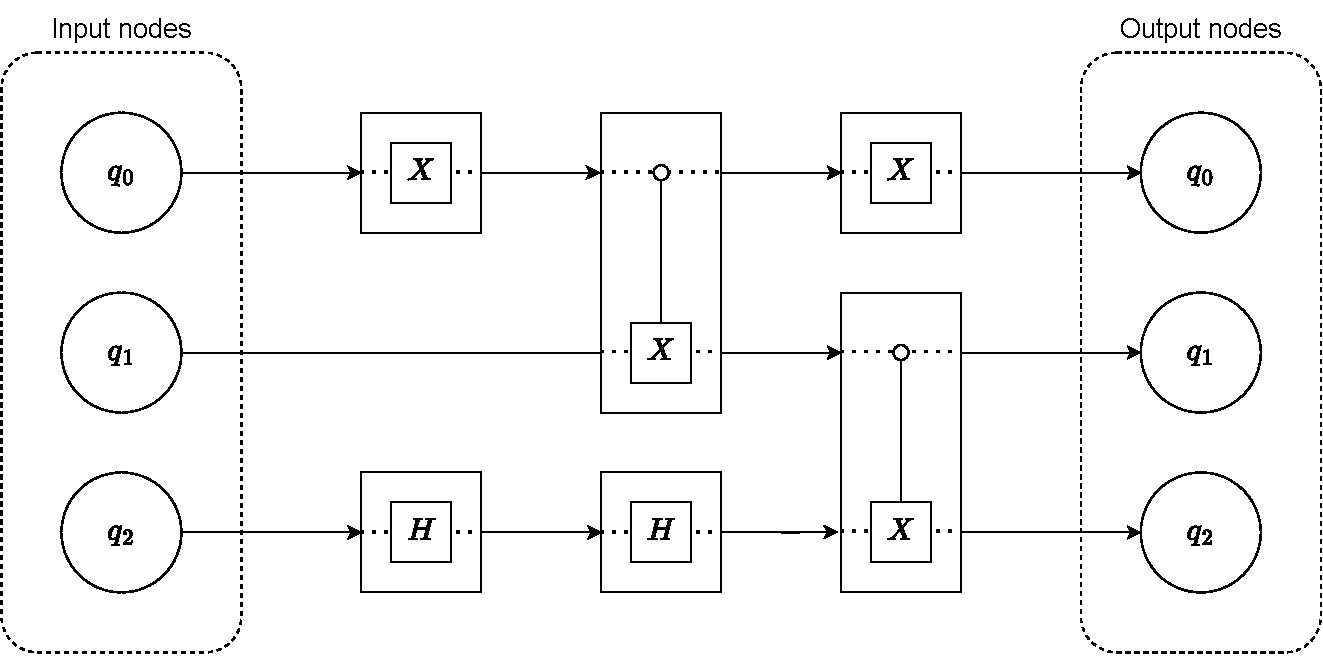
\includegraphics[width=.9\textwidth]{../figures/drawio/circuit_graph_unoptimized.pdf}
            \caption{An example of a simple, unoptimized circuit graph.}
            % \label{fig:circuit_graph_unoptimized}
        \end{figure}
    \end{minipage}
    % \begin{align*}
    %     C &= (V, E, Q, Q_E, Q_V)\\
    %     V &= \underbrace{I}_{\text{Input Nodes}} \cup \underbrace{O}_{\text{Output Nodes}} \cup \underbrace{G}_{\text{Gate Nodes}}\\
    %     E &\subseteq \{ (x, y) \mid x,y \in V \land x \neq y \}\\
    %     Q_V &: I \cup O \to Q \\
    %     Q_E &: E \to Q
    % \end{align*}
\end{frame}

% \begin{frame}{Example Circuit Graph}
%     \begin{itemize}
%         \item Input and output nodes have only one outgoing or incoming edge, respectively. 
%         \item For each qubit, $C$ contains an input-output node pair.
%         \item Each edge coming into a gate node has a corresponding outgoing one with the same qubit.
%         \item These represent an argument of the gate application.
%         \item The wire for qubit $q$ is represented by the path from the input to the output node where all edges map to $q$.
%     \end{itemize}
%     \vfill
%     \begin{minipage}{.35\textwidth}
%         \begin{figure}
%             \centering
%             \lstinputlisting[style=Luie, basicstyle=\Large\ttfamily]{../figures/code/slides/optimization_example.luie}
%             \caption{A simple, unoptimized program.}
%         \end{figure}
%     \end{minipage}
%     \begin{minipage}{.60\textwidth}
%         \begin{figure}[htp]
%             \centering     
%             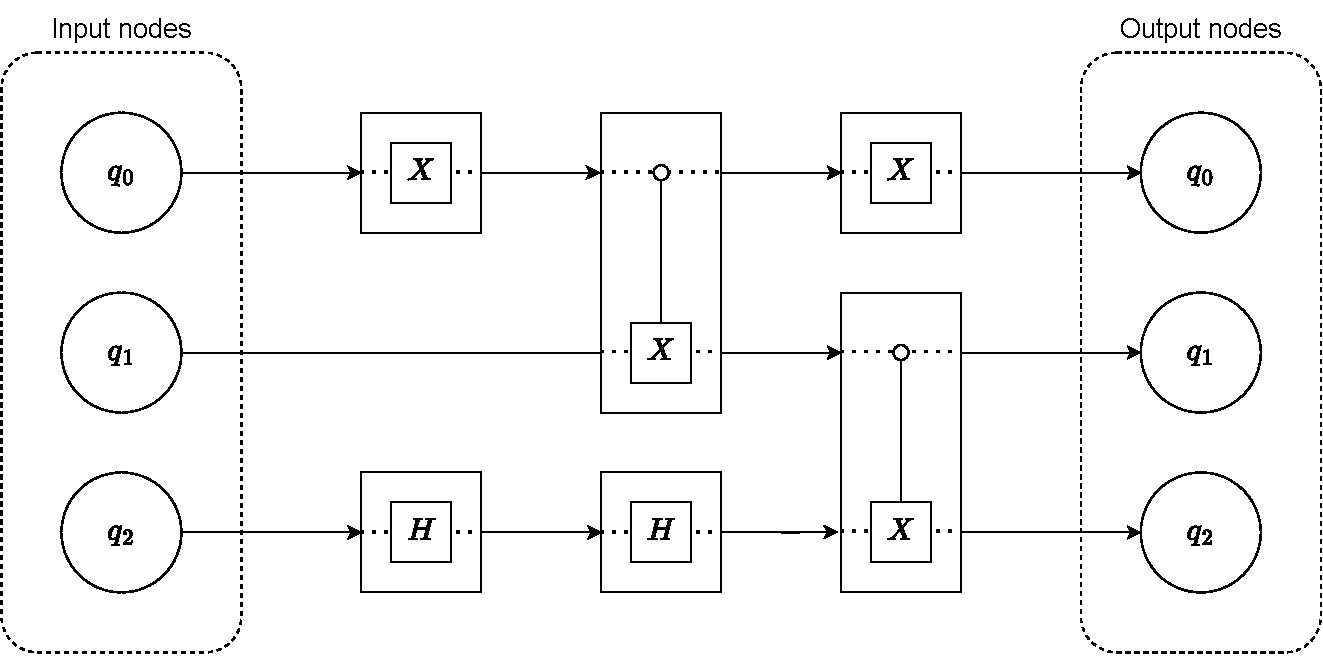
\includegraphics[width=.9\textwidth]{../figures/drawio/circuit_graph_unoptimized.pdf}
%             \caption{An example of a simple, unoptimized circuit graph.}
%             % \label{fig:circuit_graph_unoptimized}
%         \end{figure}
%     \end{minipage}
% \end{frame}

\begin{frame}{Example Optimization Process I}
    \begin{itemize}
        \item To optimize the graph, each qubit wire is iterated.
        \item All subpaths (up to max. length) checked for alternatives.
        \item Example:
        \begin{itemize}
            \item {\color{commentgreen}First wire}: Peeping control rule can be applied to first $CX$ gate.
            \item {\color{red}Third wire}: $HH$ null gate can be removed. 
        \end{itemize}
    \end{itemize}
    \vfill
    \begin{minipage}{.55\textwidth}
        \begin{figure}[htp]
            \centering     
            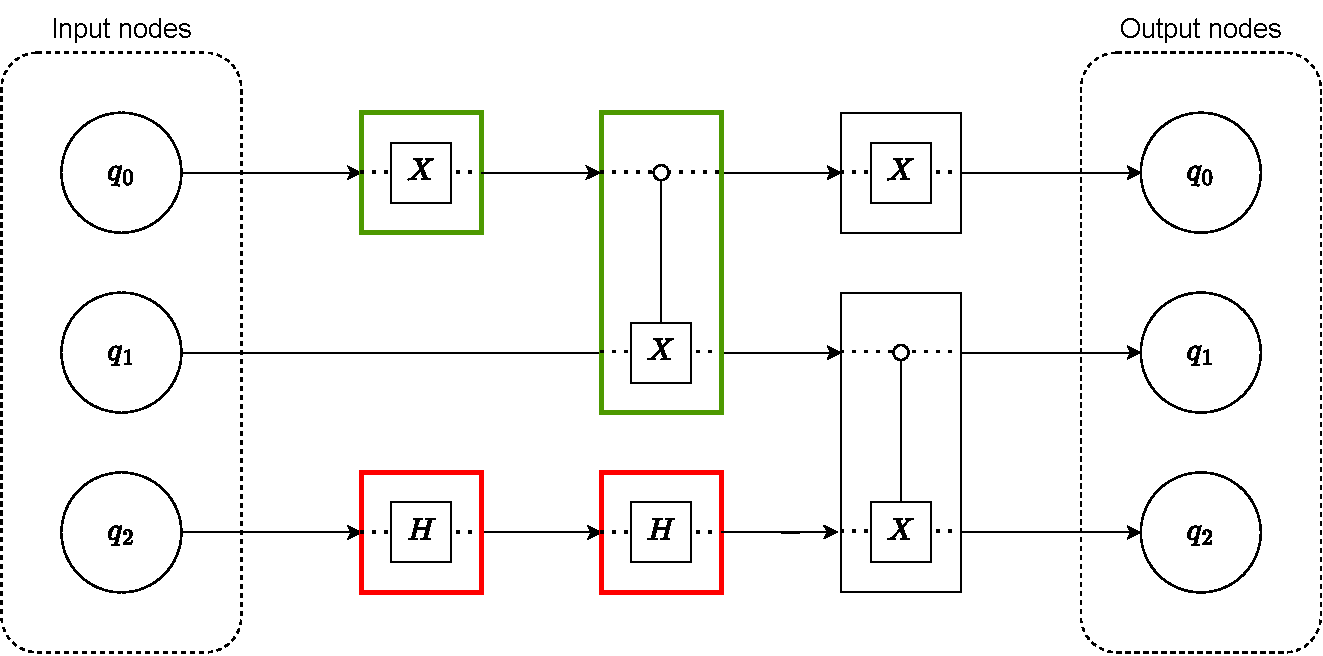
\includegraphics[width=.9\textwidth]{../figures/drawio/slides/circuit_graph_unoptimized_colored.pdf}
            \caption{An example of a simple, unoptimized circuit graph.}
            % \label{fig:circuit_graph_unoptimized}
        \end{figure}
    \end{minipage}
    \begin{minipage}{.40\textwidth}
        \begin{figure}[htp]
            \centering     
            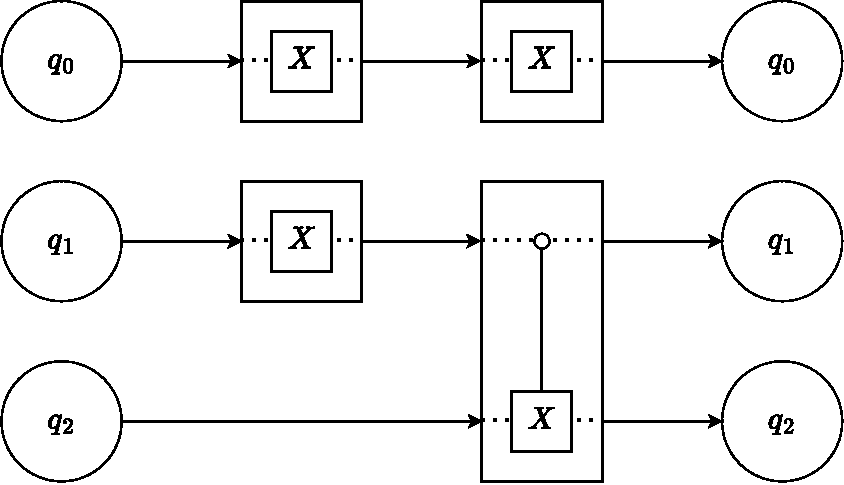
\includegraphics[width=\textwidth]{../figures/drawio/circuit_graph_optimized_firststep.pdf}
            \caption{The circuit graph after the first optimization step.}
            % \label{fig:circuit_graph_first_optimized}
        \end{figure}
    \end{minipage}
\end{frame}

\begin{frame}{Example Optimization Process II}
    \begin{itemize}
        \item While all qubit wires iterated, still possible optimizations.
        \item Applying optimizations may enable others!
        \item[$\Rightarrow$] Optimization repeated as long as previous iteration applied optimizations.
        \item Example:
        \begin{itemize}
            \item {\color{commentgreen}First wire}: $XX$ null gate can be removed.
            \item {\color{red}Second wire}: Peeping control rule can be applied to $CX$ gate.
        \end{itemize}
    \end{itemize}
    \vfill
    \hfill
    \begin{minipage}{.40\textwidth}
        \begin{figure}[htp]
            \centering     
            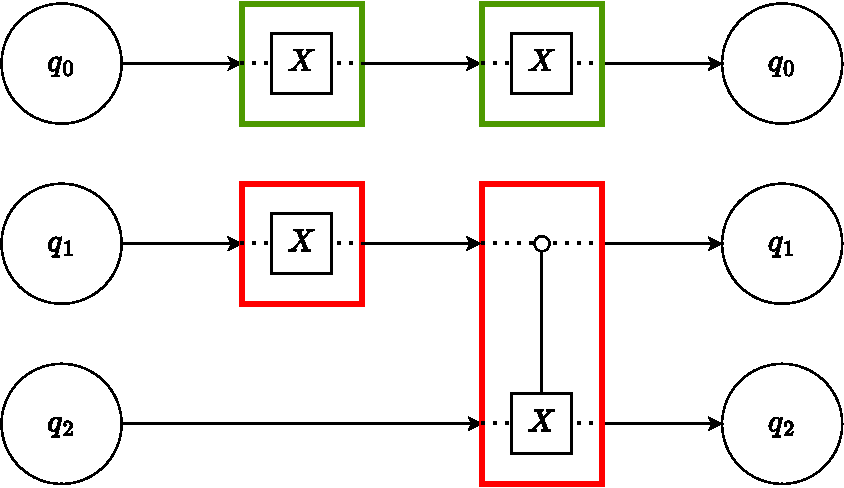
\includegraphics[width=\textwidth]{../figures/drawio/slides/circuit_graph_optimized_firststep_colored.pdf}
            \caption{The circuit graph after the first optimization step.}
            % \label{fig:circuit_graph_first_optimized}
        \end{figure}
    \end{minipage}
    \hfill
    \begin{minipage}{.30\textwidth}
        \begin{figure}[htp]
            \centering     
            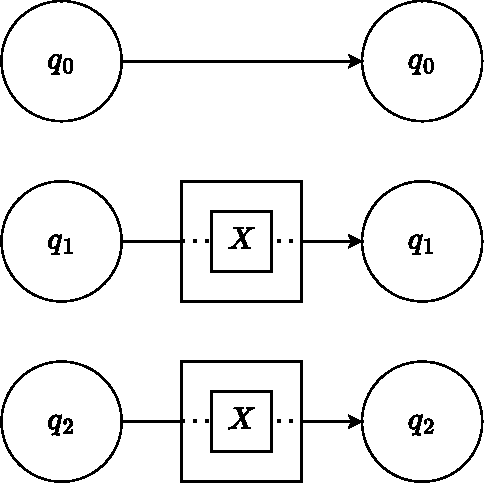
\includegraphics[width=9em]{../figures/drawio/circuit_graph_optimized_complete.pdf}
            \caption{The completely optimized graph.}
            % \label{fig:circuit_graph_optimized_complete}
        \end{figure}
    \end{minipage}
    \hfill
\end{frame}
